\documentclass[12pt,a4paper,notitlepage,twoside]{article}
\usepackage[utf8]{inputenc}
\usepackage{graphicx}
\usepackage{subcaption}
\usepackage{float}
\usepackage{listings}
\author{Robert James}
\begin{document}
\begin{Large}
\begin{center}
$02/03/15$ - $17/03/15$
\end{center}
\end{Large}

\section{Dissertation}

\begin{lstlisting}[breaklines]
eb0a68e... 2015-03-17 (23 minutes ago)
 Changes to be committed:       new file:   LabDiary/17-Mar-2015/Diary.pdf      new file:   LabDiary/17-Mar-2015/Diary.tex      new file:   LabDiary/17-Mar-2015/Diary.tex.bak  new file:   LabDiary/17-Mar-2015/q10d20/anconvergence.png       new file:   LabDiary/17-Mar-2015/q2d20/acceptance.png   new file:   LabDiary/17-Mar-2015/q2d20/anconvergence.png        new file:   LabDiary/17-Mar-2015/q2d20/energy.png       new file:   LabDiary/17-Mar-2015/q2d20/magnetisation.png        new file:   LabDiary/17-Mar-2015/q2d20/specificheat.png         new file:   LabDiary/17-Mar-2015/q2d20/susceptibility.png       new file:   LabDiary/17-Mar-2015/q4d20/anconvergence.png        new file:   ProjectReport/2015-03-02/ProjectReport.tex.bak

A       LabDiary/17-Mar-2015/Diary.pdf
A       LabDiary/17-Mar-2015/Diary.tex
A       LabDiary/17-Mar-2015/Diary.tex.bak
A       LabDiary/17-Mar-2015/q10d20/anconvergence.png
A       LabDiary/17-Mar-2015/q2d20/acceptance.png
A       LabDiary/17-Mar-2015/q2d20/anconvergence.png
A       LabDiary/17-Mar-2015/q2d20/energy.png
A       LabDiary/17-Mar-2015/q2d20/magnetisation.png
A       LabDiary/17-Mar-2015/q2d20/specificheat.png
A       LabDiary/17-Mar-2015/q2d20/susceptibility.png
A       LabDiary/17-Mar-2015/q4d20/anconvergence.png
A       ProjectReport/2015-03-02/ProjectReport.tex.bak


f1e7998... 2015-03-10 (7 days ago)
        modified:   1-Introduction/Introduction.tex     new file:   1-Introduction/Introduction.tex.bak         modified:   2-Theory/Theory.tex         new file:   2-Theory/Theory.tex.bak     new file:   2-Theory/circleandlines2.png        new file:   2-Theory/circleandlines3.png        new file:   2-Theory/circleandlines4.png        new file:   2-Theory/latticetotorus.png         new file:   2-Theory/latticetotorus.svg         new file:   2-Theory/osangersolution.png        new file:   2-Theory/q=2angles.png      new file:   2-Theory/q=2angles.svg      new file:   2-Theory/q=3angles.png      new file:   2-Theory/q=3angles.svg      modified:   Dissertation.pdf    modified:   Dissertation.tex    new file:   Dissertation.tex.bak        modified:   title.tex

M       1-Introduction/Introduction.tex
C089    1-Introduction/Introduction.tex 1-Introduction/Introduction.tex.bak
M       2-Theory/Theory.tex
A       2-Theory/Theory.tex.bak
A       2-Theory/circleandlines2.png
A       2-Theory/circleandlines3.png
A       2-Theory/circleandlines4.png
A       2-Theory/latticetotorus.png
A       2-Theory/latticetotorus.svg
A       2-Theory/osangersolution.png
A       2-Theory/q=2angles.png
A       2-Theory/q=2angles.svg
A       2-Theory/q=3angles.png
A       2-Theory/q=3angles.svg
M       Dissertation.pdf
M       Dissertation.tex
C090    Dissertation.tex        Dissertation.tex.bak
M       title.tex

a470925... 2015-03-01 (2 weeks ago)
 Changes to be committed:       new file:   LabDiary/22-Feb-2015/Diary.pdf      new file:   ProjectReport/2015-03-02/2ndDerivativeMagnetisation.PNG     new file:   ProjectReport/2015-03-02/ProjectReport.pdf  new file:   ProjectReport/2015-03-02/ProjectReport.tex  new file:   ProjectReport/2015-03-02/References.bib     new file:   ProjectReport/2015-03-02/SwanseaLogo.png    new file:   ProjectReport/2015-03-02/energyvsbeta.png   new file:   ProjectReport/2015-03-02/magnetisationvsbeta.png    new file:   ProjectReport/2015-03-02/q=3energyvsbeta.png        new file:   ProjectReport/2015-03-02/q=3magnetisationderivatives.PNG    new file:   ProjectReport/2015-03-02/q=3magnetisationvsbeta.png         new file:   ProjectReport/2015-03-02/q=4energyvsbeta.png        new file:   ProjectReport/2015-03-02/q=4magnetisationderivatives.PNG    new file:   ProjectReport/2015-03-02/q=4magnetisationvsbeta.png         new file:   ProjectReport/2015-03-02/title.tex

A       LabDiary/22-Feb-2015/Diary.pdf
A       ProjectReport/2015-03-02/2ndDerivativeMagnetisation.PNG
A       ProjectReport/2015-03-02/ProjectReport.pdf
A       ProjectReport/2015-03-02/ProjectReport.tex
A       ProjectReport/2015-03-02/References.bib
A       ProjectReport/2015-03-02/SwanseaLogo.png
A       ProjectReport/2015-03-02/energyvsbeta.png
A       ProjectReport/2015-03-02/magnetisationvsbeta.png
A       ProjectReport/2015-03-02/q=3energyvsbeta.png
A       ProjectReport/2015-03-02/q=3magnetisationderivatives.PNG
A       ProjectReport/2015-03-02/q=3magnetisationvsbeta.png
A       ProjectReport/2015-03-02/q=4energyvsbeta.png
A       ProjectReport/2015-03-02/q=4magnetisationderivatives.PNG
A       ProjectReport/2015-03-02/q=4magnetisationvsbeta.png
A       ProjectReport/2015-03-02/title.tex

\end{lstlisting}


\section{Code}

\begin{lstlisting}[breaklines]
18cd655... 2015-03-17 (32 minutes ago)
 Changes to be committed:       new file:   anconvergence/param.cfg     new file:   anconvergence/plotan.plot   new file:   anconvergence/run.sh        new file:   anconvergence/template.cfg  modified:   betatest/plotspecificheat.plot      modified:   betatest/run.sh     modified:   betatest/template.cfg       modified:   main.cpp    modified:   param.cfg   modified:   potts.cpp   modified:   potts.h

C062    param.cfg       anconvergence/param.cfg
A       anconvergence/plotan.plot
A       anconvergence/run.sh
C052    betatest/template.cfg   anconvergence/template.cfg
M       betatest/plotspecificheat.plot
M       betatest/run.sh
M       betatest/template.cfg
M       main.cpp
M       param.cfg
M       potts.cpp
M       potts.h


4ccdd3e... 2015-03-11 (6 days ago)
 Changes to be committed:       new file:   betatest/plotspecificheat.plot      new file:   betatest/plotsusceptibility.plot    modified:   betatest/run.sh     modified:   betatest/template.cfg       modified:   main.cpp    modified:   param.cfg   modified:   potts.cpp   modified:   potts.h

A       betatest/plotspecificheat.plot
A       betatest/plotsusceptibility.plot
M       betatest/run.sh
M       betatest/template.cfg
M       main.cpp
M       param.cfg
M       potts.cpp
M       potts.h


b96734e... 2015-03-10 (7 days ago)
        modified:   betatest/plotmagnetisation.plot     modified:   betatest/run.sh     renamed:    template.cfg -> betatest/template.cfg       deleted:    critical/analysis.sh        deleted:    critical/param.cfg  deleted:    critical/plotall.plot       deleted:    critical/plotenergy.plot    deleted:    critical/plotmagnetisation.plot     deleted:    critical/run.sh     modified:   main.cpp    modified:   param.cfg   modified:   potts.cpp

M       betatest/plotmagnetisation.plot
M       betatest/run.sh
R070    template.cfg    betatest/template.cfg
D       critical/analysis.sh
D       critical/param.cfg
D       critical/plotall.plot
D       critical/plotenergy.plot
D       critical/plotmagnetisation.plot
D       critical/run.sh
M       main.cpp
M       param.cfg
M       potts.cpp


0d6beaf... 2015-03-05 (12 days ago)
        modified:   betatest/plotenergy.plot    modified:   betatest/run.sh     modified:   param.cfg

M       betatest/plotenergy.plot
M       betatest/run.sh
M       param.cfg

55d2285... 2015-03-05 (12 days ago)
 Changes to be committed:       modified:   main.cpp    modified:   param.cfg   modified:   potts.cpp   modified:   potts.h     modified:   template.cfg        modified:   utilityfunctions.cpp        modified:   utilityfunctions.h

M       main.cpp
M       param.cfg
M       potts.cpp
M       potts.h
M       template.cfg
M       utilityfunctions.cpp
M       utilityfunctions.h

\end{lstlisting}

\section{Data and Results}
\subsection{Metropolis Thermodynamic Quantities}

The Specific Heat Capacity was calculated using
\begin{equation}
C_V = \frac{1}{T^2} \left[ <E^2> - <E>^2 \right]
\end{equation}

The Magnetic Susceptibility was calculated using
\begin{equation}
\chi = \frac{1}{T} \left[ <M^2> - <M>^2 \right]
\end{equation}

\subsection{q=2}
\begin{figure}[H]
\centering
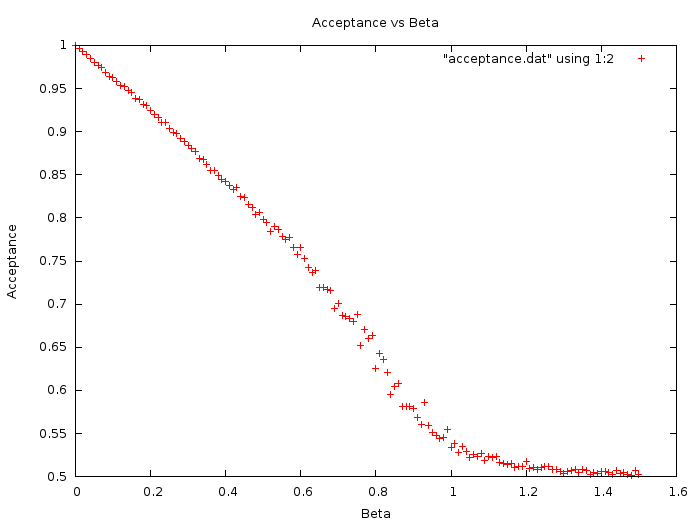
\includegraphics[width=0.4\textwidth]{q2d20/acceptance.png}
\caption{Acceptance for $q=2$ on a $20*20$ grid}
\end{figure}

\begin{figure}[H]
\centering
	\begin{subfigure}[b]{0.45\textwidth}
		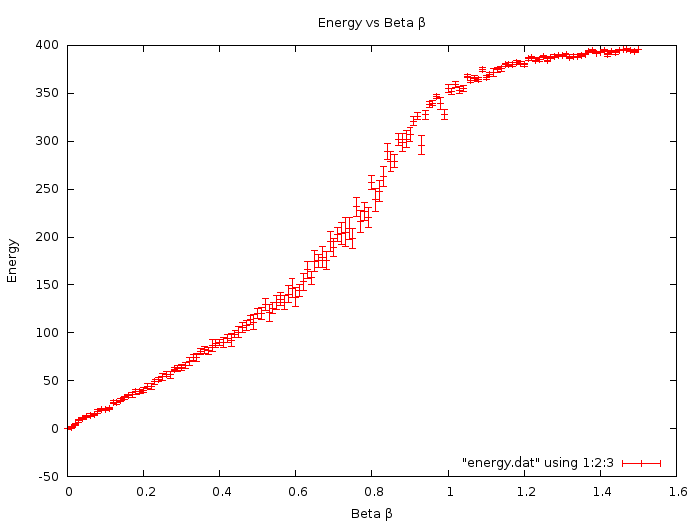
\includegraphics[width=\textwidth]{q2d20/energy.png}	
		\caption{Energy per Lattice Site with Errors}
	\end{subfigure}
	%
	\begin{subfigure}[b]{0.45\textwidth}
		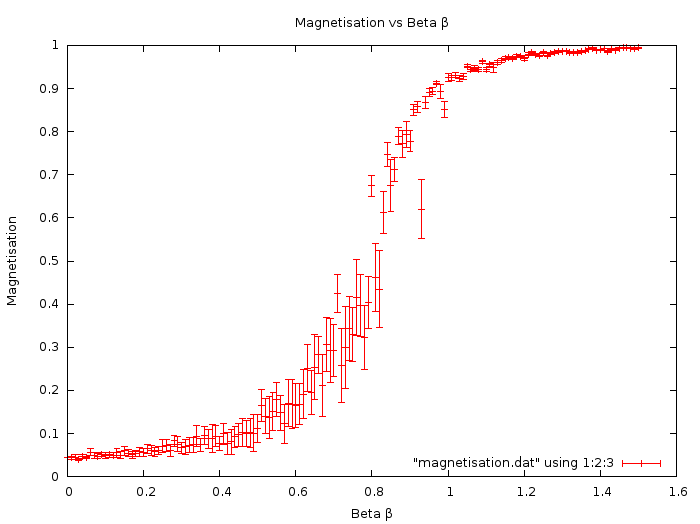
\includegraphics[width=\textwidth]{q2d20/magnetisation.png}
		\caption{Magnetisation per Lattice Site with Errors}
	\end{subfigure}
	%
\end{figure}

\begin{figure}[H]
\centering
	\begin{subfigure}[b]{0.45\textwidth}
		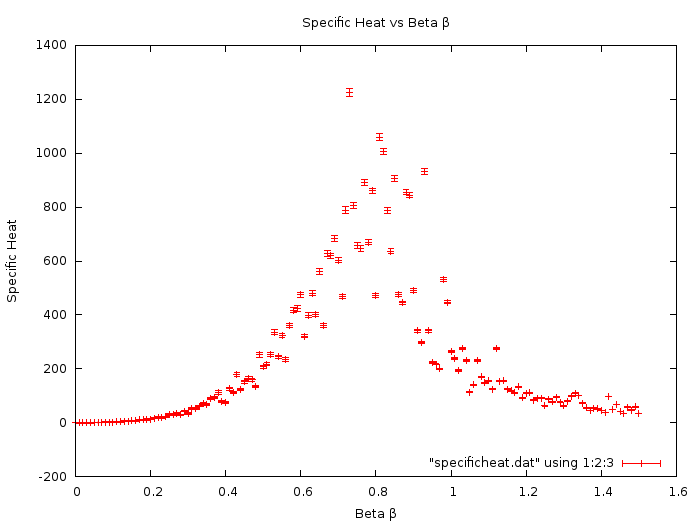
\includegraphics[width=\textwidth]{q2d20/specificheat.png}	
		\caption{Specific Heat of the System with Errors}
	\end{subfigure}
	%
	\begin{subfigure}[b]{0.45\textwidth}
		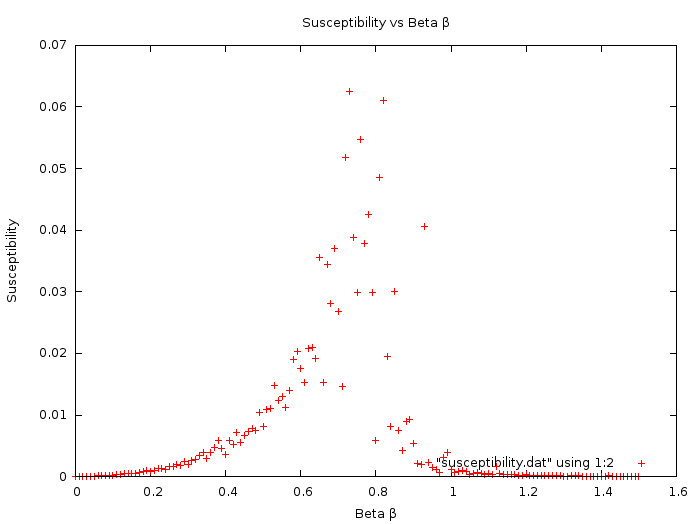
\includegraphics[width=\textwidth]{q2d20/susceptibility.png}
		\caption{Magnetic Susceptibility without errors}
	\end{subfigure}
	%
\end{figure}

\subsection{q=4}
\begin{figure}[H]
\centering
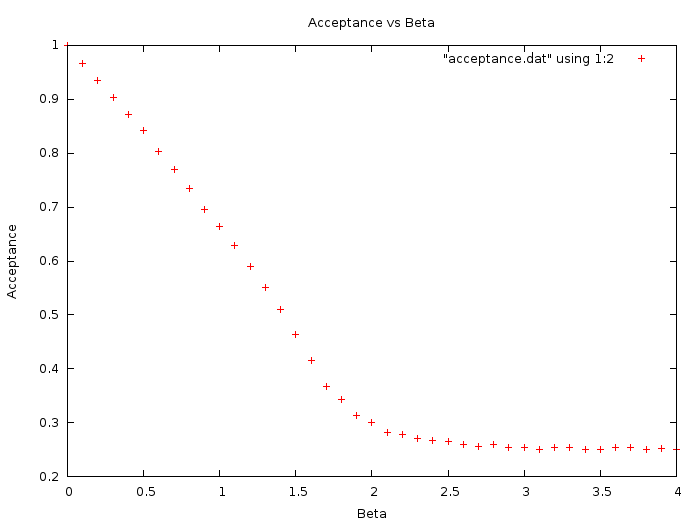
\includegraphics[width=0.4\textwidth]{q4d20/acceptance.png}
\caption{Acceptance for $q=2$ on a $20*20$ grid}
\end{figure}

\begin{figure}[H]
\centering
	\begin{subfigure}[b]{0.45\textwidth}
		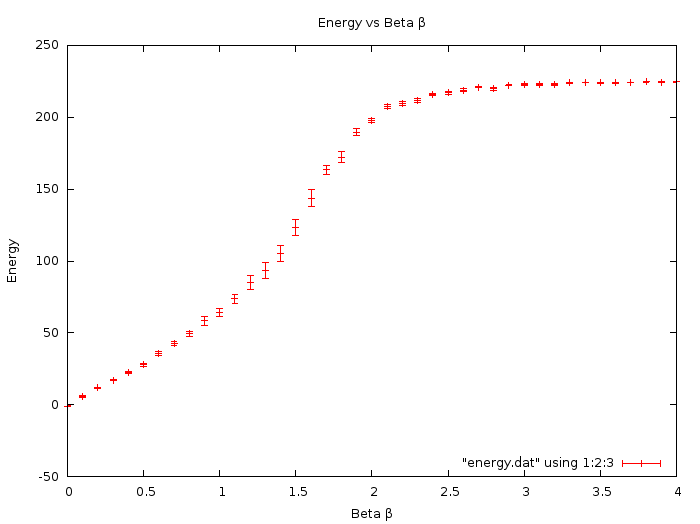
\includegraphics[width=\textwidth]{q4d20/energy.png}	
		\caption{Energy per Lattice Site with Errors}
	\end{subfigure}
	%
	\begin{subfigure}[b]{0.45\textwidth}
		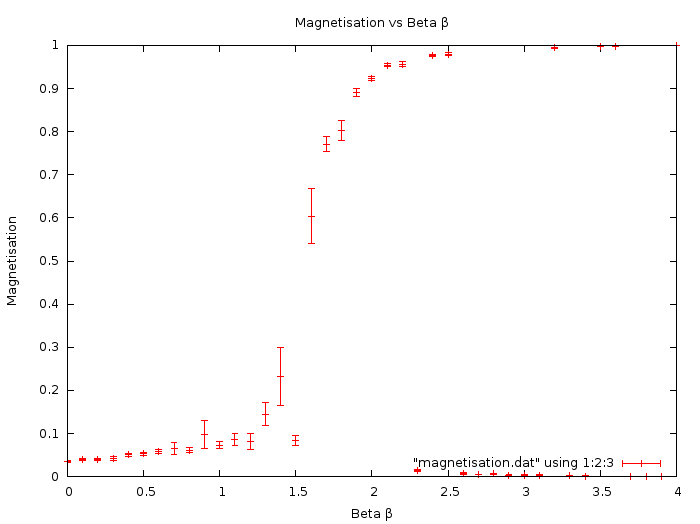
\includegraphics[width=\textwidth]{q4d20/magnetisation.png}
		\caption{Magnetisation per Lattice Site with Errors}
	\end{subfigure}
	%
\end{figure}

\begin{figure}[H]
\centering
	\begin{subfigure}[b]{0.45\textwidth}
		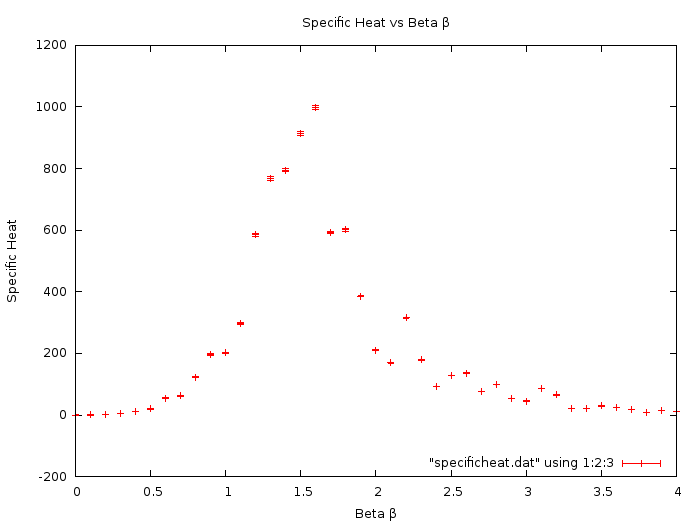
\includegraphics[width=\textwidth]{q4d20/specificheat.png}	
		\caption{Specific Heat of the System with Errors}
	\end{subfigure}
	%
	\begin{subfigure}[b]{0.45\textwidth}
		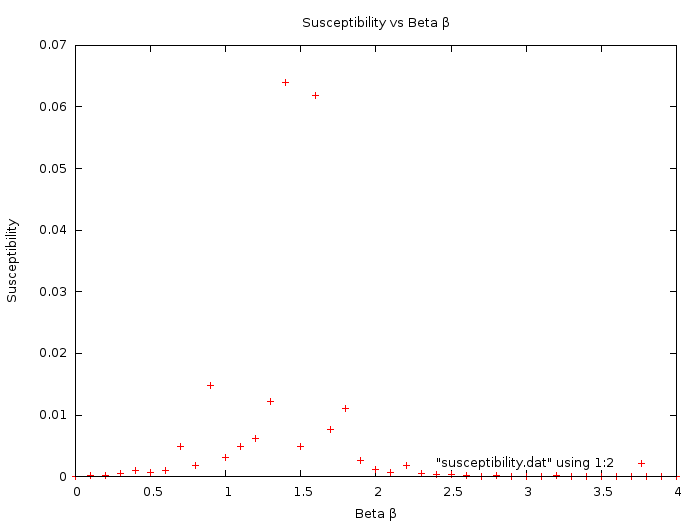
\includegraphics[width=\textwidth]{q4d20/susceptibility.png}
		\caption{Magnetic Susceptibility without errors}
	\end{subfigure}
	%
\end{figure}

\subsection{q=10}
\begin{figure}[H]
\centering
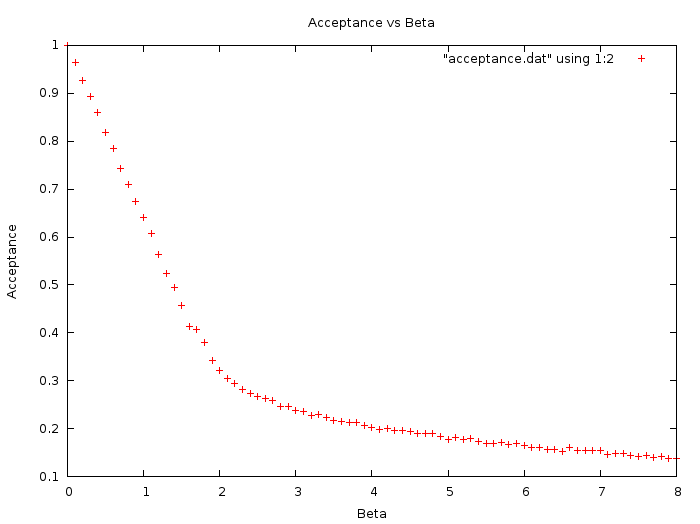
\includegraphics[width=0.4\textwidth]{q10d20/acceptance.png}
\caption{Acceptance for $q=2$ on a $20*20$ grid}
\end{figure}

\begin{figure}[H]
\centering
	\begin{subfigure}[b]{0.45\textwidth}
		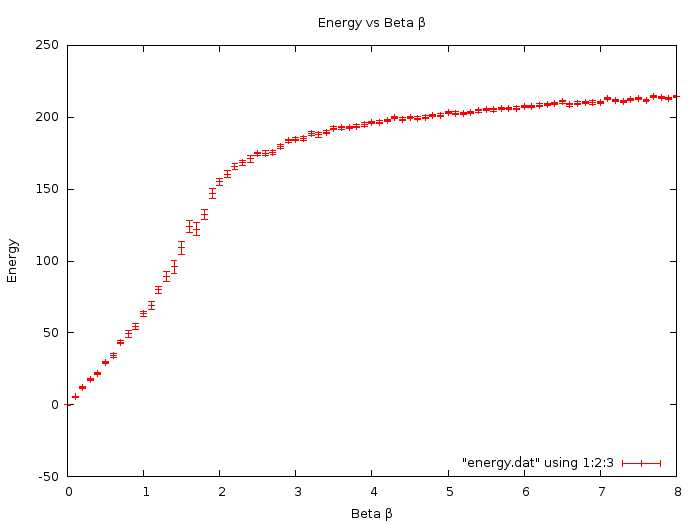
\includegraphics[width=\textwidth]{q10d20/energy.png}	
		\caption{Energy per Lattice Site with Errors}
	\end{subfigure}
	%
	\begin{subfigure}[b]{0.45\textwidth}
		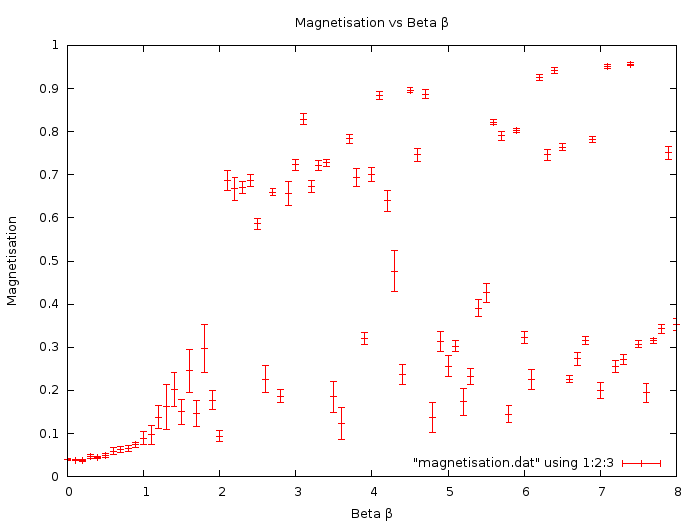
\includegraphics[width=\textwidth]{q10d20/magnetisation.png}
		\caption{Magnetisation per Lattice Site with Errors}
	\end{subfigure}
	%
\end{figure}

\begin{figure}[H]
\centering
	\begin{subfigure}[b]{0.45\textwidth}
		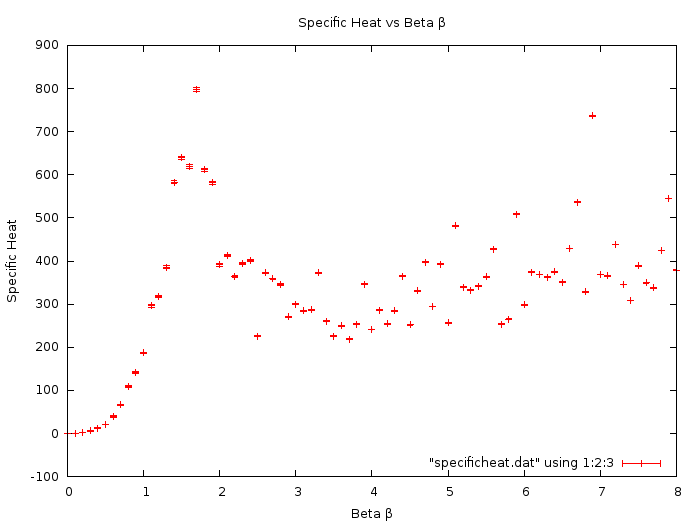
\includegraphics[width=\textwidth]{q10d20/specificheat.png}	
		\caption{Specific Heat of the System with Errors}
	\end{subfigure}
	%
	\begin{subfigure}[b]{0.45\textwidth}
		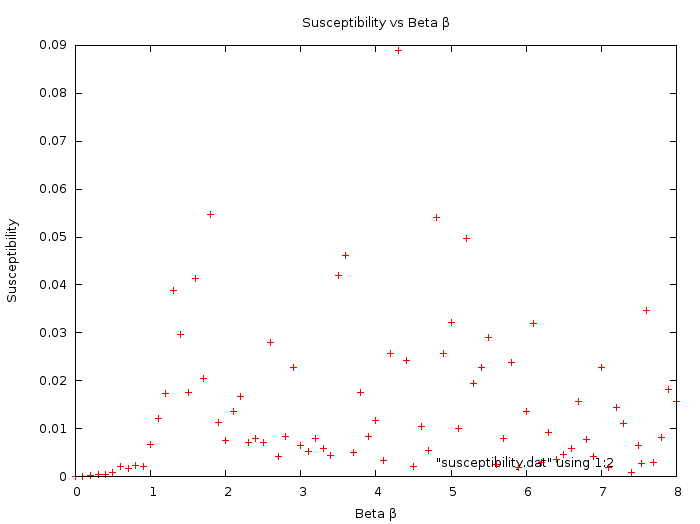
\includegraphics[width=\textwidth]{q10d20/susceptibility.png}
		\caption{Magnetic Susceptibility without errors}
	\end{subfigure}
	%
\end{figure}

At higher and higher $q$ we get some interesting artefacts after the phase transition, behaviours that look like energy level splitting and multiple minor phase transitions.

Because the Error of the Magnetic Susceptibility becomes significantly larger than the data itself around $\beta_c$ it was not shown in this plot as to show the behaviour.

Behaviour is as expected when coupling is $J = 1/2$ to match the Ising Model. However when changing to the Antiferromagnetic case $J=-0.5$ the simulation becomes erratic.
Further investigation will be required to identify the source of the problem.

\subsection{an Convergence}

\begin{figure}[H]
\centering
\begin{subfigure}[b]{0.45\textwidth}
	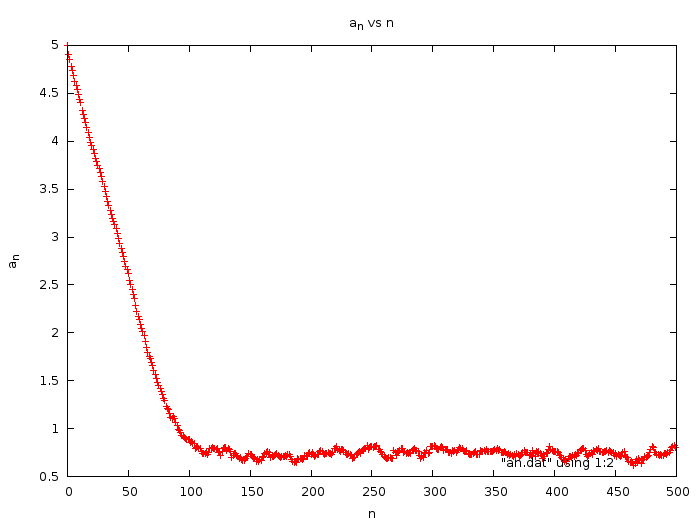
\includegraphics[width=0.9\textwidth]{q2d20/anconvergence.png}
	\caption{$q=2$}
\end{subfigure}
	%
\begin{subfigure}[b]{0.45\textwidth}
	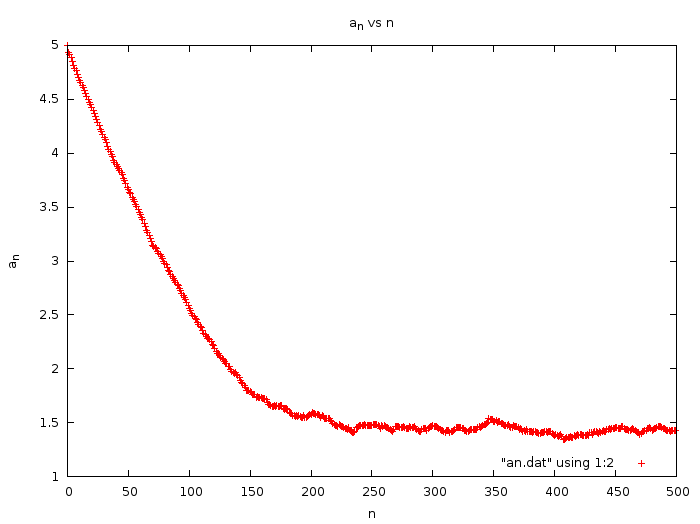
\includegraphics[width=0.9\textwidth]{q4d20/anconvergence.png}
	\caption{$q=4$}
\end{subfigure}

\begin{subfigure}[b]{0.45\textwidth}
	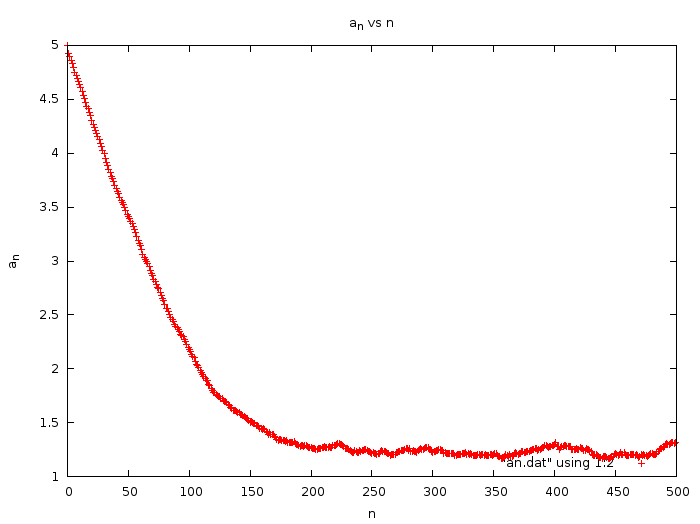
\includegraphics[width=0.9\textwidth]{q10d20/anconvergence.png}
	\caption{$q=10$}
\end{subfigure}
\caption{Target Energy: $-100.0$, Energy Band Width: $15.0$}
\end{figure}

Taking the energies calculated from the Metropolis at various $\beta$ and using those as a target to drive the configuration into to calculate $a_n$. I intend to prove that the two different values are indeed compatible.

\end{document}